\documentclass[12pt]{article}
\usepackage{scrextend}
\usepackage[utf8]{inputenc}
\usepackage[polish]{babel}
\usepackage[T1]{fontenc}%polskie znaki
\usepackage[utf8]{inputenc}%polskie znaki
\usepackage{geometry}
\usepackage{float}
\usepackage{enumitem}
\usepackage{hyperref}
\usepackage{graphicx}
\usepackage{tabulary}
\usepackage{etoc}
\usepackage[normalem]{ulem} 
\renewcommand{\baselinestretch}{1.5}
\graphicspath{ {img/} }
\newgeometry{lmargin=2.0cm, rmargin=2.0cm, tmargin=2.0cm, bmargin=2.0cm}
\usepackage{tikz}
\usepackage[bf]{caption}
\usepackage{dirtytalk}
\usepackage{listings}
\usepackage{xcolor}
\newcommand{\paragraphnewline}[1]{\paragraph{#1}\mbox{}\\}



\definecolor{codegreen}{rgb}{0,0.6,0}
\definecolor{codegray}{rgb}{0.5,0.5,0.5}
\definecolor{codepurple}{rgb}{0.58,0,0.82}
\definecolor{backcolour}{rgb}{0.95,0.95,0.92}

\lstdefinelanguage{JavaScript}{
  morekeywords=[1]{break, continue, delete, else, for, function, if, in,
    new, return, this, typeof, var, void, while, with, import, from, as, readonly, string, export, class, async, implements},
  % Literals, primitive types, and reference types.
  morekeywords=[2]{false, null, true, boolean, number, undefined,
    Array, Boolean, Date, Math, Number, String, Object, Promise},
  % Built-ins.
  morekeywords=[3]{eval, parseInt, parseFloat, escape, unescape},
  sensitive,
  morecomment=[s]{/*}{*/},
  morecomment=[l]//,
  morecomment=[s]{/**}{*/}, % JavaDoc style comments
  morestring=[b]',
  morestring=[b]"
}[keywords, comments, strings]

\lstdefinestyle{mystyle}{
    backgroundcolor=\color{backcolour},   
    commentstyle=\color{codegreen},
    keywordstyle=\color{magenta},
    numberstyle=\tiny\color{codegray},
    stringstyle=\color{codepurple},
    basicstyle=\ttfamily\footnotesize,
    breakatwhitespace=false,         
    breaklines=true,                 
    captionpos=b,                    
    keepspaces=true,                 
    numbers=left,                    
    numbersep=5pt,                  
    showspaces=false,                
    showstringspaces=false,
    showtabs=false,                  
    tabsize=2
}
\renewcommand{\lstlistlistingname}{Spis listingów}\lstset{style=mystyle}



\title{ 
    \vspace*{50mm}
    \textsc{
        \textbf{Bazy Danych 2}\\
        \large Household App - Zarządzanie gospodarstwem domowym 
    }
} 
\author{
Maja Bojarska\\
Damian Koper\\
}

%\date{14 października 2019}
\date{19 stycznia 2020}

\begin{document}

\maketitle

\newpage
\setcounter{tocdepth}{2}
\localtableofcontents
\listoffigures
\lstlistoflistings

\newpage

\section{Zespół}
Członkowie zespołu tworzącego aplikację ze wstępnym podziałem na role:
\begin{itemize}
    \item Maja Bojarska:
        \begin{itemize}
            \item Projekt, implementacja i testowanie encji bazy danych wraz z mapowaniem obiektowo-relacyjnym.
            \item Projekt, implementacja i testowanie RESTful API.
        \end{itemize}
    \item Damian Koper:
        \begin{itemize}
            \item Projekt odwzorowania obiektów świata rzeczywistego za pomocą encji w bazie danych.
            \item Projekt i implementacja interfejsu użytkownika.
            \item Testy jednostkowe i integracyjne poszczególnych komponentów systemu.
            \item Testy end-to-end interfejsu użytkownika.
        \end{itemize}
\end{itemize}

\section{Opis systemu}
Gospodarstwo domowe jest miejscem zrzeszającym domowników. Każda z osób ma wkład w jego rozwój. W celu śledzenia i równoważenia kosztów wynikających z użytkowania dostępnych zasobów potrzebny jest system śledzący i obliczający wydatki. Domownicy mogą dzielić się kosztami utrzymania po równo, lub odgórnie zdefiniować zasady określające procentowy wkład każdej osoby.

Działania te, razem ze śledzeniem zużycia mediów (woda, prąd, gaz), pozwolą na dokładniejsze przeanalizowanie wydatków. W przyszłości może się to przełożyć na bardziej świadome zarządzanie zasobami, a dzięki temu na optymalizację ponoszonych kosztów.

\newpage

\section{Wymagania funkcjonalne}

\subsection{Zarządzanie użytkownikami i gospodarstwem}

\begin{enumerate}
    \item Użytkownik może zalogować się na swoje konto.
    \item Użytkownik może wylogować się ze swojego konta.
    \item Użytkownik może edytować dane swojego konta.
    \item Administrator może utworzyć konto użytkownika.
    \item Administrator może edytować dane i rolę użytkownika.
    \item Administrator może usunąć konto użytkownika.
    \item Administrator może zmienić ustawienia procentowego udziału danego użytkownika w wydatkach gospodarstwa.
\end{enumerate}
    
\subsection{Zakupy}

\begin{enumerate}
    \item Użytkownik może wprowadzić dane zakupu przedmiotu.
    \item Użytkownik może edytować dane zakupu przedmiotu.
    \item Użytkownik może usuwać dane zakupu przedmiotu.
    \item Użytkownik może tworzyć sklepy.
    \item Użytkownik może edytować sklepy.
    \item Użytkownik może usuwać sklepy.
    \item Użytkownik może tworzyć kategorie.
    \item Użytkownik może edytować kategorie.
    \item Użytkownik może usuwać kategorie.
\end{enumerate}

\subsection{Listy zakupów}

\begin{enumerate}
    \item Użytkownik może dodać listy zakupów
    \item Użytkownik może edytować listy zakupów
    \item Użytkownik może usuwać listy zakupów
    \item Użytkownik może dodać pozycję listy zakupów.
    \item Użytkownik może edytować pozycję listy zakupów.
    \item Użytkownik może usuwać pozycję listy zakupów.
    \item Użytkownik może przekonwertować listę zakupów na wstępnie utworzone dane o zakupach.
\end{enumerate}

\subsection{Wydatki gospodarstwa}

\begin{enumerate}
    \item Uzytkownik może wprowadzić dane o jednorazowych wydatkach.
    \item Uzytkownik może edytować dane o jednorazowych wydatkach.
    \item Uzytkownik może usuwać dane o jednorazowych wydatkach.
    \item Użytkownik może wprowadzić reguły obliczeń kosztów zużycia mediów.    
    \item Użytkownik może edytować reguły obliczeń kosztów zużycia mediów.    
    \item Użytkownik może usuwać reguły obliczeń kosztów zużycia mediów.    
    \item Użytkownik może wprowadzić dane zużycia mediów.
    \item Użytkownik może edytować dane zużycia mediów.
    \item Użytkownik może usuwać dane zużycia mediów.
\end{enumerate}

\newpage

\subsection{Statystyki i raporty}

\begin{enumerate}
    \item Użytkownik może wyświetlić statystyki kosztów zakupów dla każdego użytkownika, dla ustawionego okresu:
    \begin{enumerate}
        \item Zakupy w czasie jako wykres liniowy.
        \item Zakupy zgrupowane w kategorie jako wykres kolumnowy.
        \item Procentowy udział kategorii we wszystkich zakupach jako wykres kołowy.
    \end{enumerate}
    \item Użytkownik może wyświetlić statystyki dla wszystkich zakupów lub tylko dla zakupów współdzielonych.
    \item Użytkownik może wyświetlić liczbowe podsumowanie danego miesiąca zawierające:
    \begin{enumerate}
        \item Kwoty zakupów współdzielonych podzielone na wszystkich użytkowników z uwzględnionym ustawionym podziałem.
        \item Kwoty do zapłaty dla poszczególnych użytkowników pozostałym użytkownikom wynikające z wprowadzonych zakupów i opłaconych rachunków.
    \end{enumerate}
\end{enumerate}

\section{Wymagania niefunkcjonalne}
\begin{enumerate}
    \item Aplikacja zapewnia bezpieczeństwo sesji użytkownika.
    \item Aplikacja jest odporna na popularne ataki - SQL Injection, XSS, Man in the middle.
    \item Interfejs graficzny aplikacji działa po stronie przeglądarki użytkownika i komunikuje się z jej serwerem za pomocą RESTful API.
    \item Aplikacja zapewnia spójność interfejsu z aplikacjami mobilnymi używając stylu \textit{Material Design}.
    \item Aplikacja zapewnia funkcjonalności Progressive Web App.
    \item Architektura aplikacji musi umożliwiać szybką instalację wszystkich jej komponentów, serwisów i jej uruchomienie za pomocą jednej komendy.
\end{enumerate}

\newpage
\section{Przypadki użycia}

\begin{figure}[!htb]
    \centering
    \includegraphics[keepaspectratio,
    width=\linewidth]{diagrams/out/ucd_user_management.png}
    \caption{Diagram przypadków użycia - użytkownicy.}
\end{figure}

\begin{figure}[!htb]
    \centering
    \begin{minipage}[b]{0.45\textwidth}
        \includegraphics[width=\textwidth]{diagrams/out/ucd_shop.png}
        \caption{Diagram przypadków użycia - sklepy.}
    \end{minipage}
    \hfill
    \begin{minipage}[b]{0.45\textwidth}
        \includegraphics[width=\textwidth]{diagrams/out/ucd_category.png}
        \caption{Diagram przypadków użycia - kategorie.}
    \end{minipage}
\end{figure}

\begin{figure}[!htb]
    \centering
    \includegraphics[keepaspectratio,
    width=\linewidth]{diagrams/out/ucd_shopping_list.png}
    \caption{Diagram przypadków użycia - lista zakupów.}
\end{figure}

\begin{figure}[!htb]
    \centering
    \begin{minipage}[b]{0.45\textwidth}
        \includegraphics[keepaspectratio, width=\textwidth, height=10cm]{diagrams/out/ucd_purchase.png}
        \caption{Diagram przypadków użycia - zakupy.}
    \end{minipage}
    \hfill
    \begin{minipage}[b]{0.45\textwidth}
        \includegraphics[width=\textwidth]{diagrams/out/ucd_stats_reports.png}
        \caption{Diagram przypadków użycia - statystyki.}
    \end{minipage}
\end{figure}
\clearpage
\begin{figure}[!htb]
    \centering
    \includegraphics[keepaspectratio,
    width=\linewidth,
    height=\dimexpr\textheight-2\baselineskip]{diagrams/out/ucd_expenses.png}
    \caption{Diagram przypadków użycia - wydatki.}
\end{figure}



\newpage

\section{Architektura}
Aplikacja wykorzystuje architekturę trójwarstwową, gdzie interface użytkownika, część zawierająca logikę biznesową i~baza danych stanowią oddzielne, osobno rozwijane moduły. Użytkownik ma dostęp do aplikacji poprzez przeglądarkę internetową, co przy zachowaniu responsywności interface'u, daje mu dowolność wyboru wykorzystywanego typu urządzenia. Użytkownik komunikując się z aplikacją wysyła zapytania do dwóch serwerów:
\begin{enumerate}
  \item Do serwera plików statycznych, który wysyła kod części działającej po stronie przeglądarki użytkownika - aplikacji \textit{SPA}.
  \item Do serwera zarządzającym zasobami aplikacji zapewniającym bezstanową komunikację w~stylu REST, który odpowiedzialny jest za pobieranie i~modyfikowanie stanu aplikacji.
\end{enumerate}
Podział ruchu na dwa serwery pozwala odseparować pobieranie zasobów aplikacji od zapytań ingerujących w~jej stan - przetwarzających dane, co ułatwi późniesze skalowanie aplikacji. w~późniejszych fazach rozwoju projektu serwer plików statycznych może znajdować się na innej maszynie.

\subsection{Multitenancy}
Struktura danych aplikacji nie zakłada podziału przypisania encji na wiele gospodarstw, co oznacza, że jedna baza danych może obsłużyć tylko jedno gospodarstwo. Jest to celowa konstrukcja, która zakłada w~przyszłości zastosowanie architektury multitenancy. Zakłada ona dynamiczne przekierowywanie ruchu do odpowiedniej bazy danych w~zależności od ustalonej zmiennej - np. subdomeny. Aplikacja w~zakładanej obecnie formie jest przeznaczona do instalacji \textit{on premises}.

\section{Technologie}
Baza danych aplikacji będzie działać w~oparciu o DBMS \textit{MariaDB}\cite{mariadb}, który bazuje na i~jest kompatybilny z popularnym systemem \textit{MySQL}. Serwerem plików statycznych będzie \textit{NGINX}\cite{nginx}, który jest bardziej przystępny w~konfiguracji, od stanowiącego konkurencję serwera \textit{Apache}\cite{Apache}. Zużywa on mniej zasobów oraz osiąga większą wydajność. 

Środowiskiem uruchomieniowym dla aplikacji udostępniającej RESTful API będzie \textit{NodeJS}\cite{NodeJS}. Aplikacja ta będzie oparta na frameworku \textit{NestJS}\cite{NestJS}, który pozwala na tworzenie wydajnych i~skalowalnych aplikacji z użyciem języka \textit{TypeScript}. \textit{NestJS} będzie będzie współpracował z frameworkiem \textit{TypeORM}\cite{typeorm} obsługującym mapowanie obiektowo-relacyjne.

Frontend aplikacji, przesyłany do użytkownika za pomocą serwera plików statycznych, zostanie stworzony z użyciem języka \textit{TypeScript} i~frameworka \textit{VueJS}\cite{VueJS}. Za wygląd aplikacji będzie odpowiadać framework \textit{Vuetify}\cite{Vuetify}, który zaopatruje w~gotowy zestaw komponentów, które wyglądem zgodne są ze stylem \textit{Material Design}\cite{Material Design}.

Całość uruchamiana będzie z użyciem wirtualizacji na poziomie systemu operacyjnego, z użyciem środowiska \textit{Docker}\cite{Docker}. Pozwoli to zminimalizować liczbę kroków potrzebnych do konfiguracji środowiska na różnych maszynach oraz ujednolici je na maszynach deweloperów, co poskutkuje minimalizacją błędów związanych z różnicą konfiguracji w~różnych środowiskach.

\begin{figure}[H]
  \centering
  \includegraphics[keepaspectratio, height=15cm]{diagrams/out/deployment.png}
  \caption{Diagram wdrożenia.}
\end{figure}


\section{Baza danych}

\subsection{Diagram encji}

\begin{figure}[H]
  \centering
  \includegraphics[keepaspectratio, height=15cm]{diagrams/out/entity_relationship_diagram.png}
  \caption{Diagram encji.}
\end{figure}

\newpage % Bo ładniej na nowej stronie

\subsection{Transakcje i~spójność danych}

W celu zachowania spójności danych w~bazie danych, transakcje są realizowane ograniczeniem pola\\\textit{\say{ON DELETE SET NULL}}, \textit{\say{ON DELETE CASCADE}} lub \textit{\say{ON DELETE RESTRICT}}.

\begin{enumerate}

  \item Usunięcie użytkownika powoduje:
  \begin{itemize} 
    \item  ustawienie odniesień do niego w~encji \textit{Lista zakupów} na wartość \textit{NULL}.
    \item Usunięcie zakupów, których dokonał, czyli takich, w~których jest wpisany w~pole\\\textit{boughtBy}. Jeżeli usuwany użytkownik jest wpisany w~danej krotce w~pole \textit{boughtFor}, jest ono ustawiane na wartość \textit{NULL}.
    \item Usunięcie jego wydatków.
    \item Usunięcie jego wpisów zużycia mediów.
  \end{itemize}

  \item Usunięcie listy zakupów powoduje usunięcie przedmiotów znajdujących się w~tej liście.

  \item Usunięcie sklepu powoduje ustawienie odniesień do niego w~encji \textit{Lista zakupów} na wartość \textit{NULL}.
  
  \item Encje \textit{Kategoria} i~\textit{Sklep} nie mogą zostać usunięte jeśli powiązane są z encją \textit{Zakup}.

  \item Encja \textit{Reguła obliczeń kosztów zużycia mediów} nie może zostać usunięta, jeśli jest powiązana z encją \textit{Zużycie mediów}.
  
  \item Konwersja listy zakupów na zakupy powoduje:
  \begin{itemize}
    \item Dodanie nowych krotek encji \textit{Zakup}.
    \item Usunięcie konwertowanej listy oraz wszystkich jej przedmiotów.
  \end{itemize}
\end{enumerate}

\newpage

\section{Implementacja}


\subsection{Backend}

\subsubsection{Framework Nest.js}

Backend został zbudowany z wykorzystaniem progresywnego frameworka Nest.js, opartego na języku TypeScript. Łączy on w sobie koncepcje programowania obiektowego, funkcyjnego i funkcyjno-reaktywnego. Do obsługi zapytań wykorzystuje framework Express. Nest.js umożliwia budowanie wysoce skalowalnych aplikacji, co jest dużą zaletą w kontekście realizowanego projektu. W aplikacji Household App został użyty do budowy RESTapi.

\subsubsection{Moduły aplikacji}

Aplikacja Nest.js składa się m.in. z modułów, które są wydajnym sposobem podziału aplikacji na niezależne od siebie komponenty. Za pomocą dekoratora \lstinline{@Module} określa sie z jakich kontrolerów i serwisów korzysta dany moduł. Każdy moduł może importować (wykorzystywać) również inne moduły, które są wymienione w parametrze \lstinline{imports}.

\begin{lstlisting}[language=JavaScript, caption={Implementacja modułu \lstinline{ShopsModule}.}, label=lst:nest:module]
@Module({
  imports: [
    PassportModule.register({ defaultStrategy: 'jwt' }),
    TypeOrmModule.forFeature([Shop]),
    ConfigModule,
    CategoriesModule,
  ],
  controllers: [ShopsController],
  providers: [ShopsService],
  exports: [ShopsService],
})
export class ShopsModule {}
\end{lstlisting}

\newpage
Każde powiązanie (zależność) pomiędzy dwoma modułami reprezentowane jest poprzez połączenie strzałką o przerywanej linii. Na poniższym diagramie, moduł A zależy od modułu B.

\begin{figure}[!htb]
  \centering
  \includegraphics[keepaspectratio,
    width=0.65\linewidth,
    height=\dimexpr\textheight-2\baselineskip]{diagrams/out/modules_dependency_legend.png}
  \caption{Legenda do diagramu zależności modułów.}
\end{figure}

Niektóre moduły są zależnością dla wszystkich innych modułów, które występują na poniższym diagramie. Powiązania z nimi nie zostały pokazane, w celu zachowania czytelności grafu. Są to następujące moduły:
\begin{itemize}[noitemsep]
  \item \lstinline{PassportModule}
  \item \lstinline{ConfigModule}
  \item \lstinline{TypeOrmModule}
\end{itemize}


\begin{figure}[H]
  \centering
  \includegraphics[keepaspectratio,
    width=0.8\linewidth,
    height=\dimexpr\textheight-2\baselineskip]{diagrams/out/modules_dependency.png}
  \caption{Diagram zależności modułów.}
\end{figure}

% O co chodzi w Neście itd

\subsubsection{Kontrolery}
Kontrolery odpowiadają za obsługę nadchodzących zapytań HTTP i zwracanie odpowiedzi do klienta. Mechanizm routowania, na podstawie ścieżki, decyduje o tym do którego kontrolera zostanie przekazane nadchodzące zapytanie. Każdy kontroler może obsługiwać wiele ścieżek, a każda z nich może realizować inną funkcję aplikacji. 

Listing \ref{lst:bills_controller} zawiera skrócony kod źródłowy kontrolera dla ścieżek rozpoczynających się od \mbox{\lstinline{/bills}.} Po przekierowaniu zapytania do odpowiedniej metody kontrolera obsługującej podaną ścieżkę, kontroler wykonuje potrzebne czynności poprzez dostępny mu serwis \lstinline{billsService}.

\begin{lstlisting}[language=JavaScript, caption={Implementacja kontrolera dla ścieżki \lstinline{bills}.}, label=lst:bills_controller]
  @Controller('bills')
  @ApiUseTags('bills')
  @ApiBearerAuth()
  @UseGuards(AuthGuard())
  export class BillsController {
    constructor(private readonly billsService: BillsService) {}

    @Get()
    async find() { return this.billsService.findAll(); }
  
    @Get(':id')
    async findOne(@Param('id') id: number) {
      return this.billsService.findById(id);
    }

    @Post()
    async store(@Body() createBillDto: CreateBillDto) {[...]}
  
    @Put(':id')
    async update(@Param('id') id: number, @Body() updateBillDto: UpdateBillDto) {[...]}
  
    @Delete(':id')
    async delete(@Param('id') id: number) {[...]}
  }
  \end{lstlisting}

\subsubsection{Serwisy}

Serwisy enkapsulują i dodają warstwę abstrakcji nad logikę wykorzystywaną w modułach. Głównym celem stosowania serwisów jest wstrzykiwanie zależności do innych klas. Każdy serwis jest klasą odekorowaną dekoratorem \lstinline{@Injectable()}, implementującą określony zestaw metod.

\begin{lstlisting}[language=JavaScript, caption={Implementacja serwisu \lstinline{ShopsService}.}, label=lst:nest:service]
@Injectable()
export class ShopsService {
  constructor(
    @InjectRepository(Shop)
    private readonly shopRepository: Repository<Shop>,
    private readonly categoriesService: CategoriesService,
  ) {}

  async findAll(): Promise<Shop[]> {
    return await this.shopRepository.find({relations: ['defaultCategory']});
  }

  async findById(id: number): Promise<Shop | undefined> {
    const shop = await this.shopRepository.findOne(id);
    if (!shop) {
      throw new NotFoundException();
    }
    return shop;
  }

  async create(dto: CreateShopDto): Promise<Shop> {[...]}

  async update(id: number, dto: UpdateShopDto): Promise<Shop> {[...]}

  async delete(id: number): Promise<Shop> {[...]}
}
  \end{lstlisting}

\newpage
\subsubsection{Obsługa zapytania}

Poniższy diagram prezentuje przepływ informacji podczas wywołania zapytania HTTP do \mbox{RESTapi.}

\begin{figure}[H]
  \centering
  \includegraphics[keepaspectratio,
    width=\linewidth,
    height=\dimexpr\textheight-2\baselineskip]{diagrams/out/nest_request_flow.png}
  \caption{Diagram sekwencji przepływu informacji podczas obsługi zapytania.}
\end{figure}

\newpage
\subsubsection{Struktura RESTapi}

RESTapi dla każdej encji pozwaja na operacje pobierania, dodawania, edycji i usuwania. Wykorzystuje do tego metody protokołu HTTP oraz odpowiednio skonstruowane adresy.

\begin{itemize}[noitemsep]
  \item \lstinline{GET /nazwa-encji}: pobieranie wszystkich encji.
  \item \lstinline|GET /nazwa-encji/{id}|
  : pobieranie encji o podanym id.
  \item \lstinline{POST /nazwa-encji}: wprowadzanie encji.
  \item \lstinline|PUT /nazwa-encji/{id}|: aktualizowanie encji o podanym id.
  \item \lstinline|DELETE /nazwa-encji/{id}|: usuwanie encji o podanym id.
  \item \lstinline|GET /users/{id}/payments|: pobieranie należności użytkownika o podanym id.
  \item \lstinline|GET /users/{id}/purchases|: pobieranie zakupów użytkownika o podanym id.
  \item \lstinline|GET /users/{id}/shopping-lists|: pobieranie list zakupów użytkownika o podanym id.
  \item \lstinline|GET /users/{id}/expenses|: pobieranie wydatków użytkownika o podanym id.
  \item \lstinline|GET /users/{id}/bills|: pobieranie wydatków użytkownika o podanym id.
  \item \lstinline|GET /shopping-lists/{id}/shopping-list-items|: pobranie przedmiotów z listy zakupów o podanym id.
  \item \lstinline|GET /shopping-lists/{id}/to-purchases|: zamiana przedmiotów listy zakupów o podanym id, na zakupy.
\end{itemize}

\subsubsection{Walidacja pól zapytania}
Pola zapytania HTTP walidowane są poprzez stosowanie klas jawnie opisujących oczekiwanych typów, liczności, jak i konieczności ich podania. Dekorator \lstinline{ApiModelProperty} dodaje i manipuluje danymi pól modelu RESTapi, tworzonego w oparciu o framework Swagger (\ref{section:swagger}).

\begin{lstlisting}[language=JavaScript, caption={Data transfer object dla operacji tworzenia instancji encji \lstinline{Category}.}, label=lst:shops_service]
export class CreateCategoryDto {
  @ApiModelProperty({ example: 'Obuwie' })
  readonly name: string;

  @ApiModelProperty({ format: 'Hex', example: '#BADA55' })
  readonly color: string;

  @IsBoolean()
  @IsOptional()
  @ApiModelProperty({ example: false, default: false, required: false })
  readonly isShared: boolean;
}
\end{lstlisting}

%  - Pipes - validacja DTO https://docs.nestjs.com/pipes#class-validator

\subsubsection{Niestandardowe dekoratory}
Nest.js pozwala na tworzenie niestandardowych dekoratorów, które mogą być wykorzystane przy obsłudze zapytań. Listing \ref{lst:authuser} przedstawia implementację dekoratora \lstinline{AuthUser}, który umożliwia pobranie użytkownika wykonującego zapytanie.

\begin{lstlisting}[language=JavaScript, caption={Dekorator \lstinline{AuthUser}.}, label=lst:authuser]
export const AuthUser = createParamDecorator((data, req) => {
  return req.user;
});
\end{lstlisting}

\subsubsection{Uwierzytelnianie}
Podczas pomyślnego logowania, użytkownik otrzymuje token. Wylogowanie użytkownika powoduje umieszczenie jego tokena na czarnej liście, przez co staje się on nieważny (linia 36). Sesja jest aktywna, dopóki token jest ważny, tzn. dopóki istnieje i nie jest umieszczony na czarnej liście.

\begin{lstlisting}[language=JavaScript, caption={Serwis \lstinline{AuthService}.}, label=lst:auth_service]
@Injectable()
export class AuthService {
  constructor(
    private readonly jwtService: JwtService,
    private readonly userService: UsersService,
    @InjectRepository(JwtBlacklistEntry)
    private readonly jwtBlacklistEntryRepository: Repository<JwtBlacklistEntry>,
  ) { }

  async validateUser(
    createSessionDto: CreateSessionDto,
  ): Promise<User | undefined> {
    const user = await this.userService.findForAuth(createSessionDto.username);
    const valid = await bcryptjs.compare(
      createSessionDto.password,
      user.password,
    );
    if (valid) {
      return user;
    } else {
      throw new NotFoundException();
    }
  }

  async login(user: User) {
    const payload = {
      username: user.username,
      sub: user.id,
      isAdmin: user.isAdmin,
    };
    return {
      access_token: this.jwtService.sign(payload),
    };
  }

  async logout(user: User, token: string) {
    const entry = this.jwtBlacklistEntryRepository.create({
      user,
      token,
    });
    this.jwtBlacklistEntryRepository.save(entry);
  }
}
\end{lstlisting}

\subsubsection{Autoryzacja}
Użytkownik z aktywną sesją może korzystać z dostępnych mu funkcjonalności. Token jest walidowany przed obsługą każdego zapytania za pomocą klasy \lstinline{JwtStrategy} (listing \ref{lst:jwt_strategy}). 

\begin{lstlisting}[language=JavaScript, caption={Klasa \lstinline{JwtStrategy}.}, label=lst:jwt_strategy]
@Injectable()
export class JwtStrategy extends PassportStrategy(Strategy) {
  constructor(
    private readonly configService:ConfigService,
    private readonly userService:UsersService,
    @InjectRepository(JwtBlacklistEntry)
    private readonly jwtBlacklistEntryRepository:Repository<JwtBlacklistEntry>,
  ) {
    super({
      jwtFromRequest: ExtractJwt.fromAuthHeaderAsBearerToken(),
      ignoreExpiration: false,
      secretOrKey: configService.createJwtOptions().secret,
      passReqToCallback: true,
    });
  }
  async validate(req: Request, payload: any, done: (result: boolean) => void) {
    const token = /.*Bearer *(\S+)$/.exec(req.headers.authorization)[1];
    const blacklisted =
      (await this.jwtBlacklistEntryRepository.count({ token })) !== 0;
    if (blacklisted) {
      done(false);
    } else {
      return {
        id: payload.sub,
        username: payload.username,
        isAdmin: payload.isAdmin,
      }; } } }
\end{lstlisting}

\subsubsection{Mapowanie obiektowo-relacyjne}
Mapowanie obiektowo-relacyjne realizowane jest poprzez framework TypeORM. Relacja obiektu z bazą oraz innymi encjami określana jest przez klasę z dekoratorem \lstinline{@Entity()}. Listing \ref{lst:entity_category} przedstawia implementację encji \lstinline{Category}. TypeORM umożliwia m.in. zdefiniowanie relacji 1:M, poprzez użycie dekoratora \lstinline{@OneToMany()}. Ponadto przeprowadza migrację zdefiniowanych encji do bazy danych, co znacząco upraszcza proces tworzenia oprogramowania. Nie jest to jednak zalecane w środowisku produkcyjnym, ze względu na ryzyko przypadkowego naruszenia integralności bazy danych.
\newpage
\begin{lstlisting}[language=JavaScript, caption={Encja \lstinline{Category}.}, label=lst:entity_category]
@Entity()
export class Category {
  @PrimaryGeneratedColumn()
  public id?: number;
  @Column()
  public name?: string;
  @Column({ length: 7 })
  public color?: string;
  @Column({ type: 'bool', default: false, nullable: false })
  public isShared?: boolean;
  @OneToMany(type => Purchase, purchase => purchase.category, {
    onDelete: 'RESTRICT',
  })
  public purchases: Purchase[];
  @OneToMany(type => Shop, shop => shop.defaultCategory, {
    onDelete: 'RESTRICT',
  })
  public shops: Shop[]; 
}
\end{lstlisting}

Tak przygotowana encja można zostać zaimportowana jako moduł \lstinline{TypeOrmModule}.

\begin{lstlisting}[language=JavaScript, caption={Moduł \lstinline{CategoriesModule}.}, label=lst:entity_module]
@Module({
  imports: [
    PassportModule.register({ defaultStrategy: 'jwt' }),
    TypeOrmModule.forFeature([Category]),
    ConfigModule,
  ],
  controllers: [CategoriesController],
  providers: [CategoriesService],
  exports: [CategoriesService],
})
export class CategoriesModule {}
\end{lstlisting}

%  - Database - typeorm, wygląd encji, podpięcie pod moduł, wzorzec repozytorium kontra activeobject

\subsubsection{Wzorzec strażnika jako metoda kontroli dostępu}
Nest.js pozwala na użycie wzorca strażnika. Jako że w aplikacji Household App występują dwa rodzaje użytkowników, nie-administrator i administrator, konieczne było ograniczenie dostępu dla tego pierwszego rodzaju. Takie ograniczenie realizuje klasa \lstinline{AdminGuard} w listingu \ref{lst:admin_guard}. Wykorzystanie jej w definicji metody kontrolera, powoduje ograniczenie jej dostępności do grupy użytkowników będących administratorami. Przykładowo, metodę \lstinline{delete} z listingu \ref{lst:use_guards} może wywołać tylko administrator.  

\begin{lstlisting}[language=JavaScript, caption={Klasa \lstinline{AdminGuard}.}, label=lst:admin_guard]
@Injectable()
export class AdminGuard implements CanActivate {
  canActivate(
    context: ExecutionContext,
  ): boolean | Promise<boolean> | Observable<boolean> {
    const request = context.switchToHttp().getRequest();
    const user = request.user;
    return user && user.isAdmin;
  }
}
\end{lstlisting}

\begin{lstlisting}[language=JavaScript, caption={Użycie strażnika \lstinline{AdminGuard}.}, label=lst:use_guards]
@Delete(':id')
@UseGuards(AdminGuard)
async delete(@Param('id') id: number) {
  const user = await this.usersService.delete(id);
  return user;
}
\end{lstlisting}

%RESTapi, konstrukcja endpointów, GET PUT POST DELETE, przykłady

% Opisany przykład każdego elementu z overview
% https://docs.nestjs.com/first-steps
%  - Controller
%  - Provider - czyli nasz serwis
%  - Opakowanie to w moduł

\subsubsection{Swagger} \label{section:swagger}

Swagger jest frameworkiem wspierającym proces tworzenia i dokumentacji usług webowych RESTapi. Jest on zgodny ze standardem OpenAPI, który określa sposób opisu informacji przekazywanych do/z usługi RESTapi. Pozwala na szybkie testowanie i szczegółowy podgląd działania poszczególnych punktów końcowych. Rysunek \ref{ss:swagger_gui} przedstawia reprezentację struktury punktów końcowych kontrolera \textit{users}. Rysunek \ref{ss:swagger_query} przedstawia wywołanie punktu końcowego \lstinline{/users/id/purchases}, dla użytkownika o id=1.

\begin{figure}[H]
  \centering
  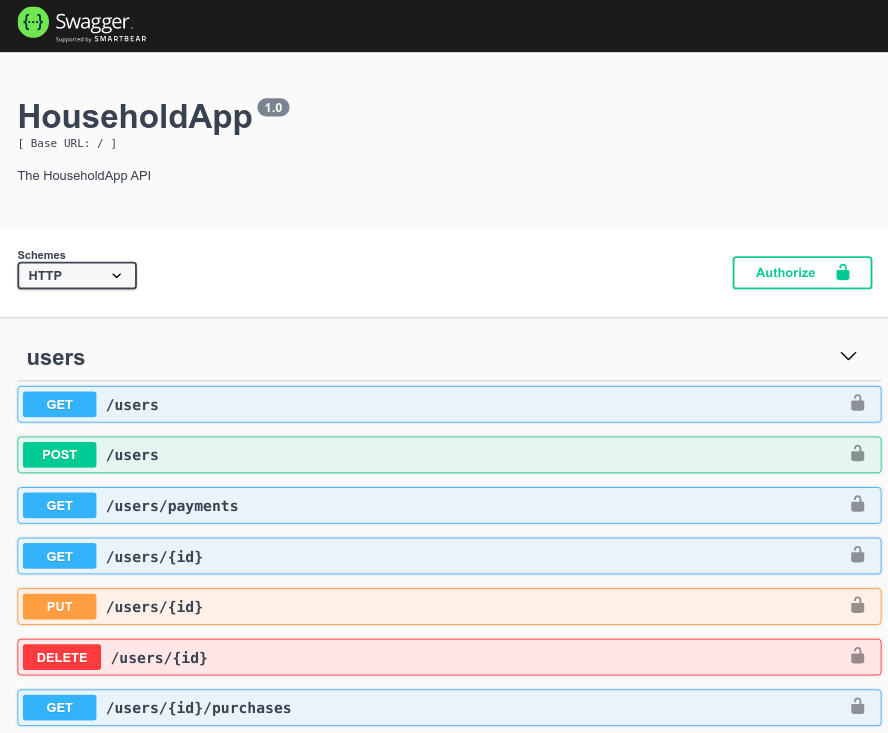
\includegraphics[keepaspectratio,
    width=\linewidth,
    height=\dimexpr\textheight-2\baselineskip]{screenshots/swagger_1.png}
  \caption{Swagger - widok struktury RESTapi.}
  \label{ss:swagger_gui}
\end{figure}


\begin{figure}[H]
  \centering
  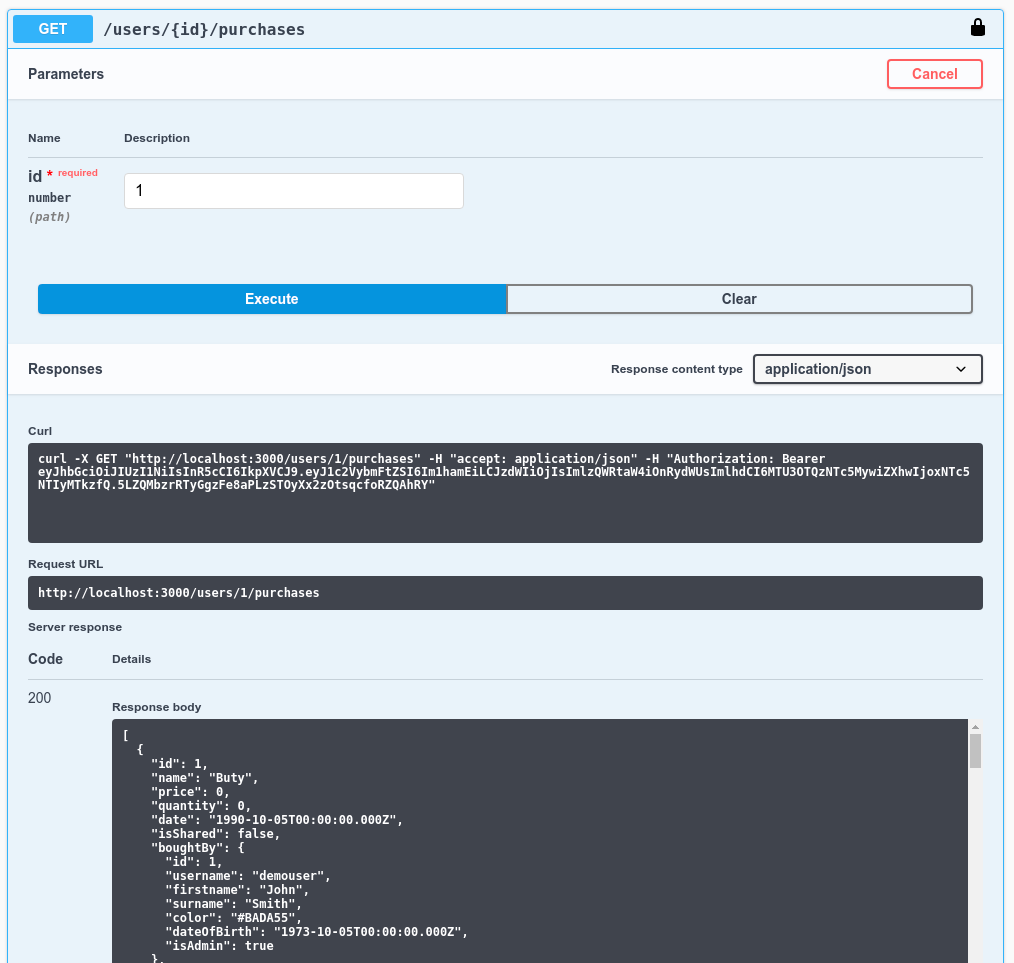
\includegraphics[keepaspectratio,
    width=\linewidth,
    height=\dimexpr\textheight-2\baselineskip]{screenshots/swagger_2.png}
  \caption{Swagger - wywołanie punktu końcowego.}
  \label{ss:swagger_query}

\end{figure}



% Swagger wisienką na torcie https://docs.nestjs.com/recipes/swagger

\newpage
\subsection{Frontend}
Interface użytkownika został napisany używając frameworka SPA VueJs. Za wygląd i funkcjonowanie komponentów odpowiedzialny był framework Vuetify, który dostarcza komponenty w stylu Material Design.

\subsubsection{Routing i podstawowe ścieżki}

Aplikacja posiada dwa zagnieżdżone routery. Pierwszy steruje głównym widokiem i przełącza pomiędzy widokiem logowania, a widokiem pozostałej części aplikacji. Drugi z nich, zawarty w widoku aplikacji, odpowiada za przełączanie widoku aplikacji pod wpływem wybieranie pozycji z menu. Listing \ref{lst:init} przedstawia kod inicjujący aplikację poprzez podanie obiektów konfiguracyjnych routera, store'a, Vuetify oraz funkcji renderującej, która jako argument przyjmuje główny komponent aplikacji - \lstinline{App}

\begin{lstlisting}[language=JavaScript, caption={Punkt wejścia skryptu inicjującego aplikację.}, label=lst:init]
import App from "./App.vue";
import router from "./router";
import store from "./store";
import vuetify from "./plugins/vuetify";
new Vue({
  router,
  store,
  vuetify,
  render: h => h(App)
}).$mount("#app");
\end{lstlisting}

Rysunek \ref{ss:login} i \ref{ss:dashboard} przedstawiają kolejno stronę logowania i pozostałą część aplikacji. Obszarem działania zagnieżdżonego routera jest obszar prawej części ekranu na rysunku \ref{ss:dashboard}.

\begin{figure}[H]
  \centering
  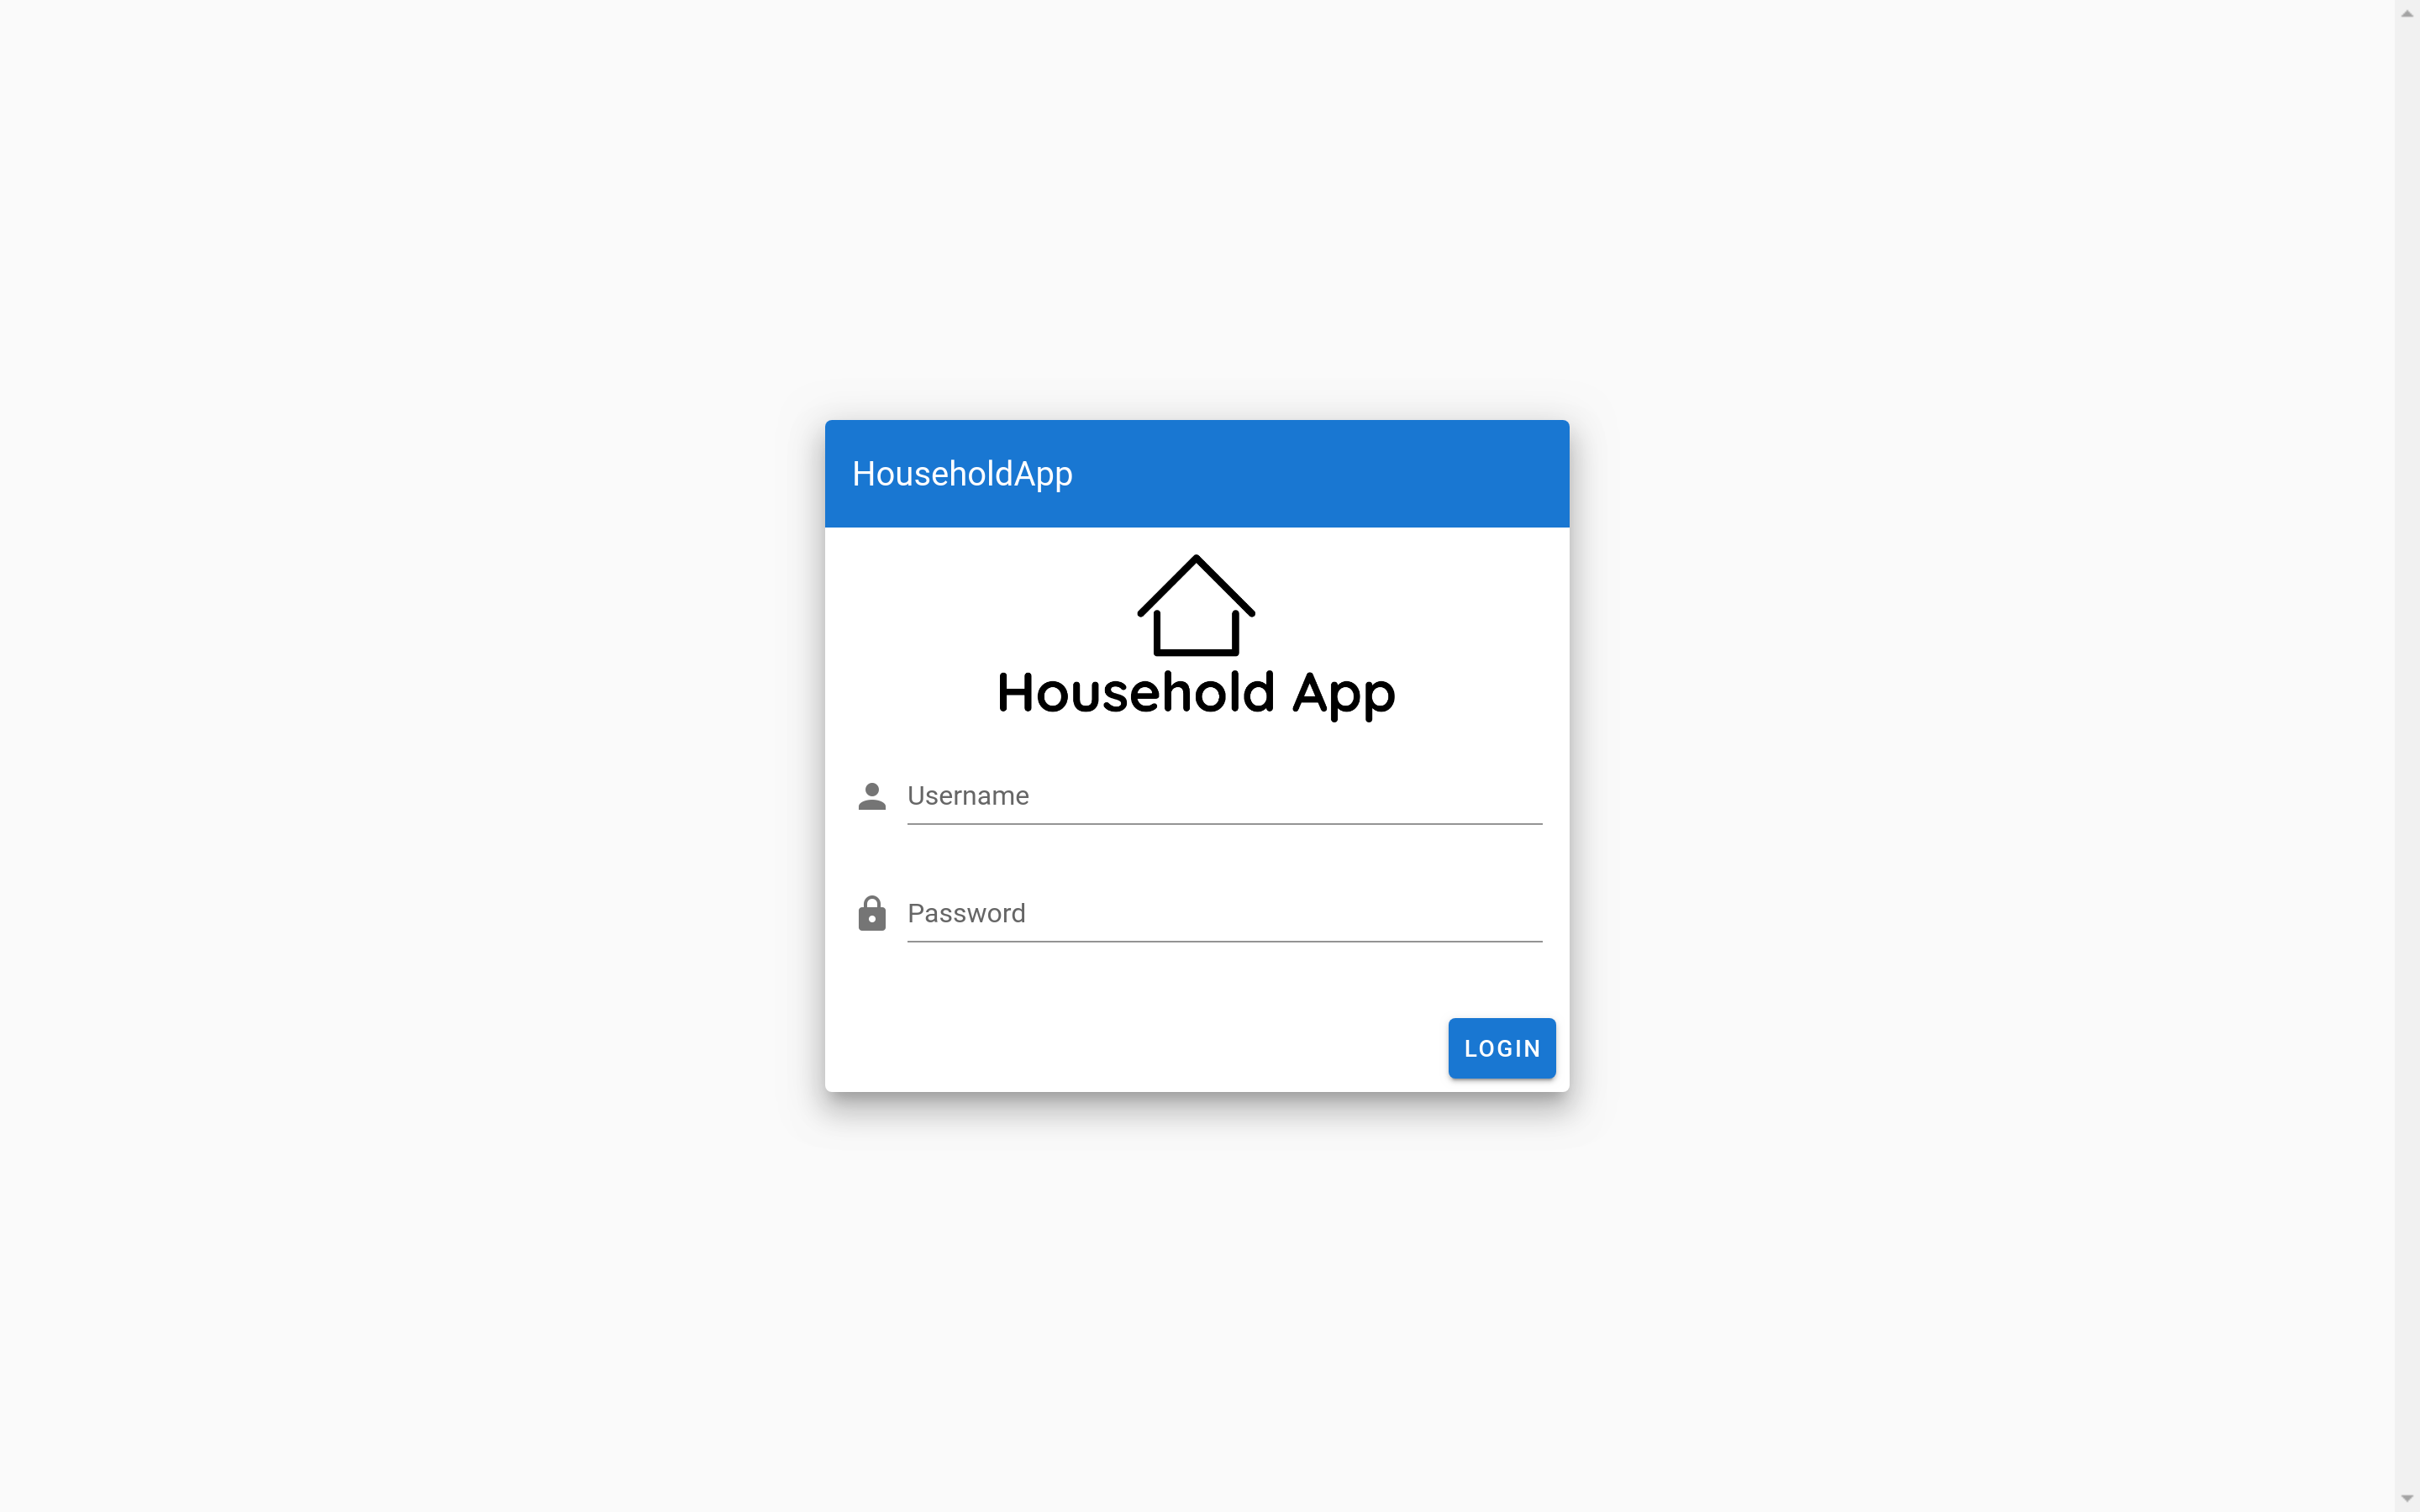
\includegraphics[width=0.95\linewidth]{screenshots/login}
  \caption{Widok strony logowania (\lstinline{/login}).}
  \label{ss:login}
\end{figure}
\begin{figure}[H]
  \centering
  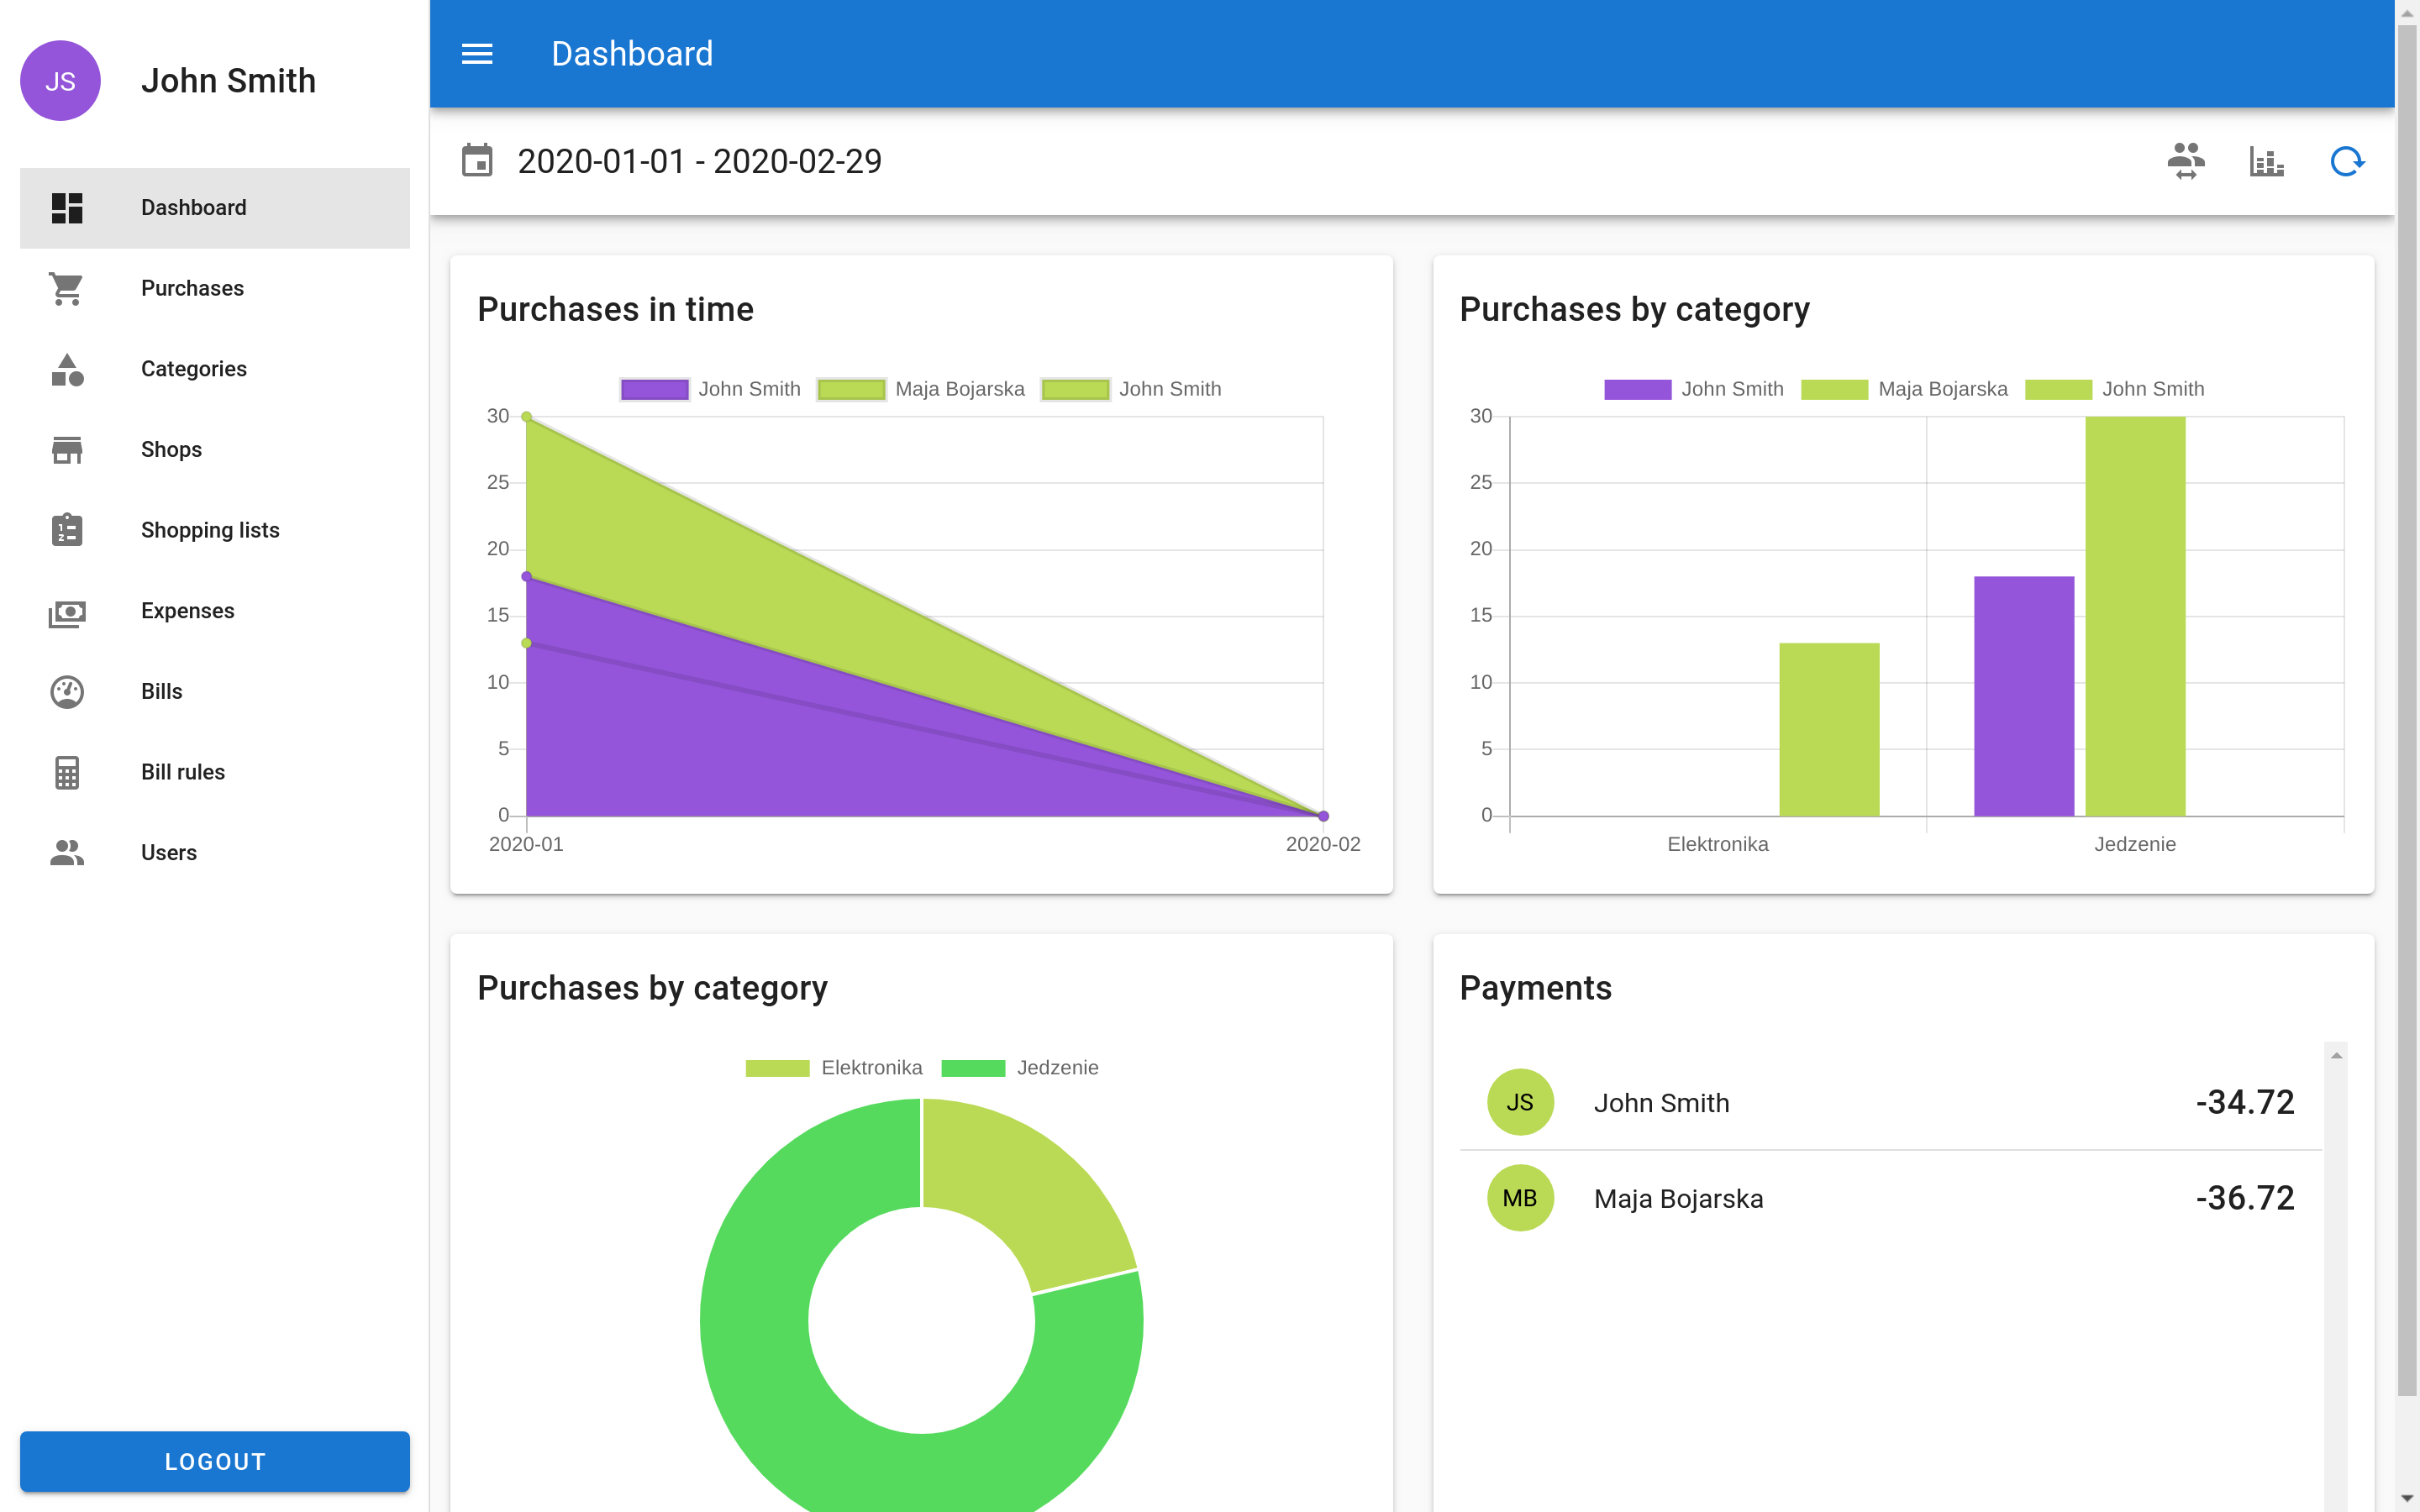
\includegraphics[width=0.95\linewidth]{screenshots/dashboard}
  \caption{Widok podsumowania (\lstinline{/dashboard}).}
  \label{ss:dashboard}
\end{figure}

\subsubsection{Komunikacja z serwerem}

Do konfiguracji z serwerem wykorzystana została biblioteka \lstinline{Axios}, która po konfiguracji adresu i portu wysyłała zapytania HTTP. Konfigurację i przykładowe zapytania zamieszczono na listingu \ref{lst:axios}.
\begin{lstlisting}[language=JavaScript, caption={Axios - konfiguracje i przykładowe użycie.}, label=lst:axios]
axios.defaults.baseURL = `http://${process.env.VUE_APP_API_URL}:${process.env.VUE_APP_API_PORT}`;
...
axios
  .get("expenses", { headers: { Authorization: this.authHeader } })
  .then((response: AxiosResponse) => {
    this.expenses = response.data;
  });
\end{lstlisting}

Na listingu \ref{lst:axios} widać również przekazywanego z każdym zapytanie wymagającym uwierzytelnienia nagłówka \lstinline{Authorization} o treści \lstinline{Bearer <TOKEN>}, gdzie \lstinline{<TOKEN>} jest tokenem otrzymanym wcześniej w procesie uwierzytelniania.

\subsubsection{Wyświetlanie i edycja danych}

Dane wyświetlane są w postaci list (rysunek \ref{ss:list}). Pozycję z listy można dodać i edytować za pomocą komponentu formularza, który pojawia się na ekranie jako okno dialogowe (rysunek \ref{ss:dialog}).

\begin{figure}[H]
  \centering
  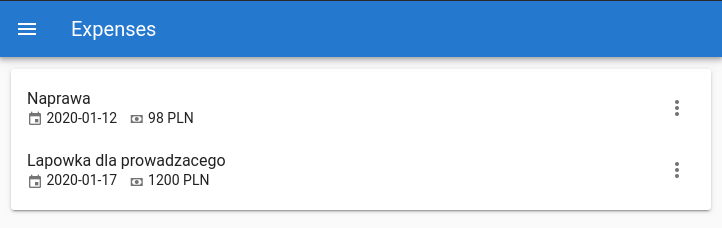
\includegraphics[width=0.8\linewidth]{screenshots/list}
  \caption{Lista wydatków (\lstinline{/expenses}).}
  \label{ss:list}
\end{figure}
\begin{figure}[H]
  \centering
  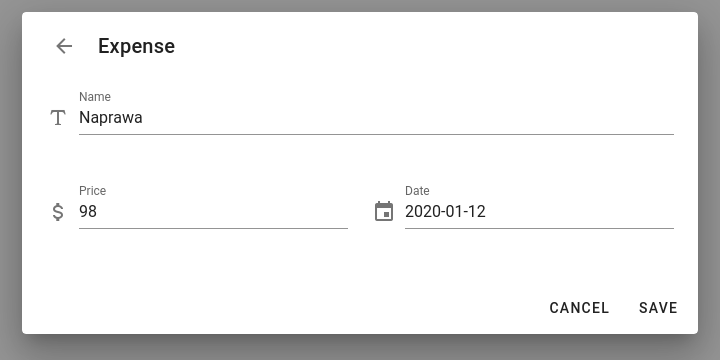
\includegraphics[width=0.8\linewidth]{screenshots/dialog}
  \caption{Edycja wydatku (\lstinline{/expenses}).}
  \label{ss:dialog}
\end{figure}

Widok listy, z pominięciem danych, definiowany jest w szablonie komponentu pokazanym na listingu \ref{lst:list}. Komponenty frameworka Vuetify charakteryzuje prefix \lstinline{v-}. Na owym listingu widać również osadzony komponent \lstinline{expense-form}, który wyświetlany jest jako ciało okna dialogowego.

\begin{lstlisting}[language=HTML, caption={Struktura widoku listy z pominięciem wyświetlania danych.}, label=lst:list]
<template>
  <v-container>
    <v-card v-if="expenses.length > 0">
      <v-list>
        <v-list-item v-for="expense in expenses" :key="expense.id"
          @click.stop="edit(expense)" >
          <v-list-item-content>
            <v-list-item-title>...</v-list-item-title>
            <v-list-item-subtitle>...</v-list-item-subtitle>
          </v-list-item-content>
          <v-list-item-action @click.stop>...</v-list-item-action>
        </v-list-item>
      </v-list>
      <v-snackbar v-model="snackbarVisible">...</v-snackbar>
    </v-card>
    <v-card v-else>...</v-card>
    <v-dialog
      v-model="dialogVisible" 
      max-width="800px"
      :fullscreen="$vuetify.breakpoint.xsOnly"
    >
      <expense-form
        :expense="dialogExpense"
        @close="dialogVisible = false"
        :type="formType"
        @submit="submit"
      />
    </v-dialog>
    <v-btn @click="create" color="primary" fab fixed right bottom>
      <v-icon>mdi-plus</v-icon>
    </v-btn>
  </v-container>
</template>
\end{lstlisting}

\subsubsection{Walidacja danych}
Za walidację danych odpowiedzialny jest komponent \lstinline{v-form}, którego obiekt posiada metodę \mbox{\lstinline{validate()}}. Walidacja wykonuje się również po każdorazowej zmiany wartości pól formularza. Komponent analizuje wartość wszystkich komponentów-dzieci wykonując na nich zdefiniowane przez aplikację reguły. Są one zdefiniowane jako jako funkcje, przyjmujące jako argument wartość pola i zwracające wartość \lstinline{true} przy poprawnej jego wartości, albo ciąg znaków z komunikatem błędu. Metodę \lstinline{validate()} odpowiedzialna jest również za wyświetlanie komunikatów użytkownikowi.
Listing \ref{lst:validation} pokazuje użycie komponentu pola tekstowego, a listing \ref{lst:validationRules} rozwinięcie reguły jego walidacji. Rysunek \ref{ss:validation} przedstawia komunikat błędu walidacji.

\begin{lstlisting}[language=HTML, caption={Komponent pola tesktowego}, label=lst:validation]
<v-text-field
  v-model="editExpense.name"
  label="Name"
  prepend-icon="mdi-format-text"
  :rules="rules.required"
/>
\end{lstlisting}
\newpage
\begin{lstlisting}[language=JavaScript, caption={Obiekt reguł walidacji.}, label=lst:validationRules]
readonly rules = {
  required: [(v: string) => !!v || "Field is required!"]
};
\end{lstlisting}

\begin{figure}[H]
  \centering
  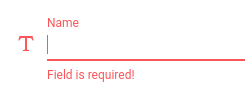
\includegraphics[width=0.3\linewidth]{screenshots/validation}
  \caption{Walidacja pola tekstowego danych edycji wydatku (\lstinline{/expenses}).}
  \label{ss:validation}
\end{figure}

\subsubsection{MVVM - Model, View, ViewModel}
Każdy komponent widoku i formularza w swojej klasie posiada zdefiniowane pola, które zawierają wyświetlane i edytowalne pola obiektów. Przykładem tego jest komponent widoku \lstinline{Expenses}, który zawiera tablicę obiektów \lstinline{Expence}. Obiekty te stanowią model widoku (ViewModel). Obiekty klas odpowiedzialne za działanie tych komponentów pośredniczą w wymianie danych pomiędzy widokiem, czyli wyświetlanym formularzem bądź listą, a modelem widoku (View <-> ViewModel). Modelem w tej relacji jest encja zapisana w bazie danych i synchronizowana a modelem widoku w momencie wywołania zdarzeń zapisania i odczytania danych z serwera \cite{mvvm}.

\newpage
\begin{thebibliography}{9}
    \bibitem{mariadb} 
    MariaDB: \url{https://mariadb.org/}
    \bibitem{nginx} 
    NGINX: \url{https://www.nginx.com/}
    \bibitem{Apache} 
    Apache: \url{https://httpd.apache.org/}
    \bibitem{NodeJS} 
    NodeJS: \url{https://nodejs.org/en/}
    \bibitem{NestJS} 
    NestJS: \url{https://nestjs.com/}
    \bibitem{typeorm}
    TypeORM: \url{https://typeorm.io/}
    \bibitem{VueJS} 
    VueJS: \url{https://vuejs.org/}
    \bibitem{Vuetify} 
    Vuetify: \url{https://vuetifyjs.com/en/}
    \bibitem{Material Design} 
    Material Design: \url{https://material.io/design/}
    \bibitem{Docker}
    Docker: \url{https://www.docker.com/}
    \bibitem{mvvm}
    MVVM: \url{https://en.wikipedia.org/wiki/Model%E2%80%93view%E2%80%93viewmodel}
\end{thebibliography}

\end{document}
